
\documentclass[mathserif,11pt]{beamer}

\mode<presentation>
{
\usetheme{default}
}


\title[] % (optional, use only with long paper titles)
{My fantastic academic talk}
% \subtitle
% {Include Only If Paper Has a Subtitle}

\author[Falster, Falster]
{
  Daniel~Falster\inst{1} \and
  \textcolor{green!50!black}{Daniel~Falster}\inst{2}
}

\institute[Macquarie University, latex land and others]
{
  \inst{1}%
  Macquarie University, Australia
  \and
  \vskip-2mm
  \inst{2}%
  latex land, Earth
}


% Includes for frame package
\usepackage{framed,color}
\definecolor{shadecolor}{rgb}{0.5,0.5,0.5}

% Make a custom block
\newenvironment<>{customBlock}[1]{%
  \begin{actionenv}#2%
      \def\insertblocktitle{#1}%
      \par%
      \mode<presentation>{%
        \setbeamercolor{block title}{fg=white,bg=orange!20!black}
       \setbeamercolor{block body}{fg=black,bg=olive!50}
       \setbeamercolor{itemize item}{fg=orange!20!black}
       \setbeamertemplate{itemize item}[triangle]
     }%
      \usebeamertemplate{block begin}}
    {\par\usebeamertemplate{block end}\end{actionenv}}


% Define new environments for mdframed package
\usepackage{tikz}
\usepackage[framemethod=tikz]{mdframed}


\newmdenv[tikzsetting={draw=black,fill=white,fill opacity=0.7, line width=4pt},backgroundcolor=none,leftmargin=0,rightmargin=0,innertopmargin=4pt,skipbelow=\baselineskip,%
skipabove=\baselineskip]{TitleBox}
%http://tex.stackexchange.com/questions/38281/transparent-background-for-mdframed-environment

\usepackage{fontawesome} 

%----------------------------------------------------------------------------------------
\begin{document}

{% My fancy title page, using transparent text box from mdframe, and icons from fontawesome
  \usebackgroundtemplate{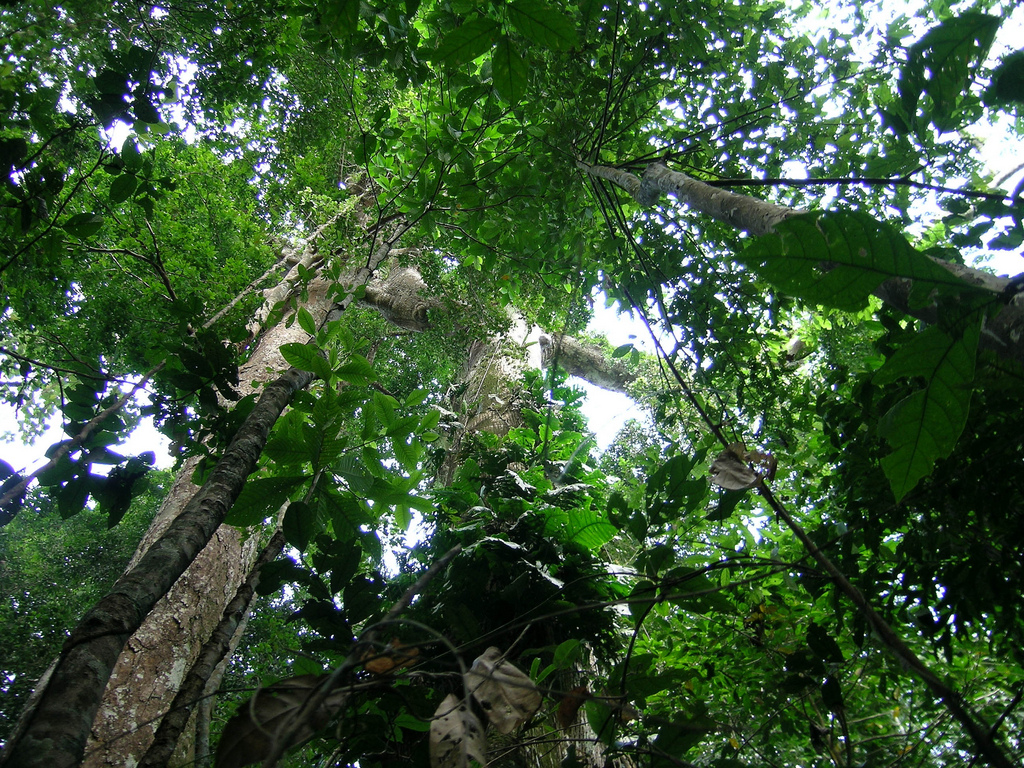
\includegraphics[width=1.0\paperwidth]{images/Background.jpg}}
  \begin{frame}[plain] 

  \vspace{15em}

  \begin{TitleBox}
    {\huge \inserttitle} 
    
    Daniel Falster, Macquarie University, Australia\\
    {\footnotesize \href{http://twitter.com/adaptive_plant}{{\FA \faTwitter} adaptive\_plant}
    \href{http://www.falsters.net/daniel}{{\FA \faHome} www.falsters.net/daniel}
    \href{mailto: daniel.falster@mq.edu.au}{{\FA \faEnvelope}  daniel.falster@mq.edu.au}
    }
   \end{TitleBox}

  \end{frame}
}


{% 
  \usebackgroundtemplate{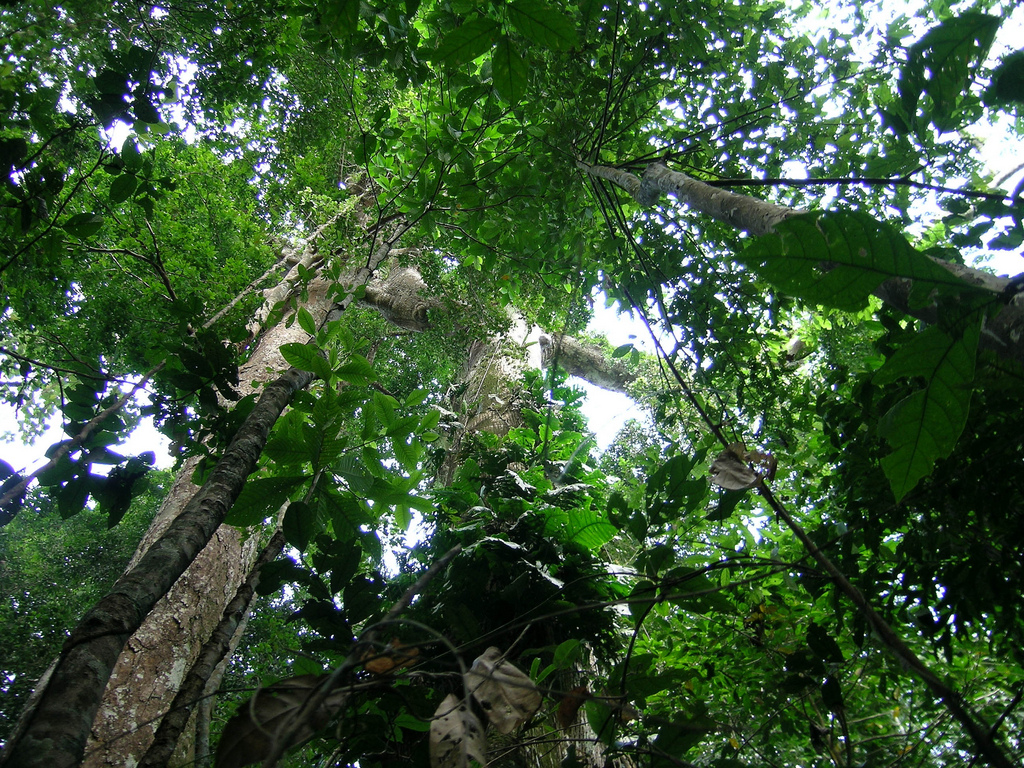
\includegraphics[width=1.0\paperwidth]{images/Background.jpg}}
  \begin{frame}[plain] 

  \begin{shaded}
  Different types of framed text. \\
  This one is a block made with frame package
  \end{shaded}

  \begin{customBlock}{A customized  block}
    Using block option
  \end{customBlock}

  \begin{mdframed}[outerlinewidth=3,leftmargin=0,%
rightmargin=20,backgroundcolor=white,%
outerlinecolor=black,innertopmargin=2pt,%
splittopskip=\topskip,skipbelow=\baselineskip,%
skipabove=\baselineskip]
  A custom frame made with mdframed, with options set locally
  \end{mdframed}

  \begin{TitleBox}
  A custom frame made with new md environment (via mdframed), and transparnecy via tikz
  \end{TitleBox}

  \end{frame}
}

{% Example using built-in title functions
  \usebackgroundtemplate{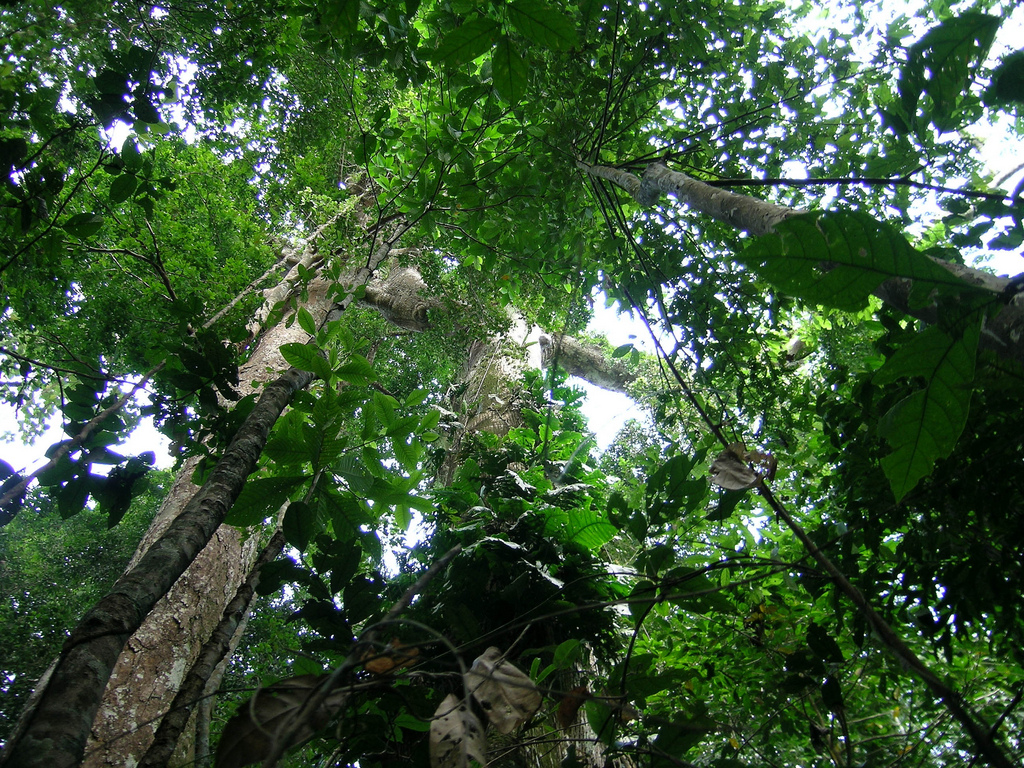
\includegraphics[width=1.0\paperwidth]{images/Background.jpg}}
  \begin{frame}[plain] 

  \begin{TitleBox}
  \maketitle  
  \end{TitleBox}

  \end{frame}
}

{%title with image as background
  \usebackgroundtemplate{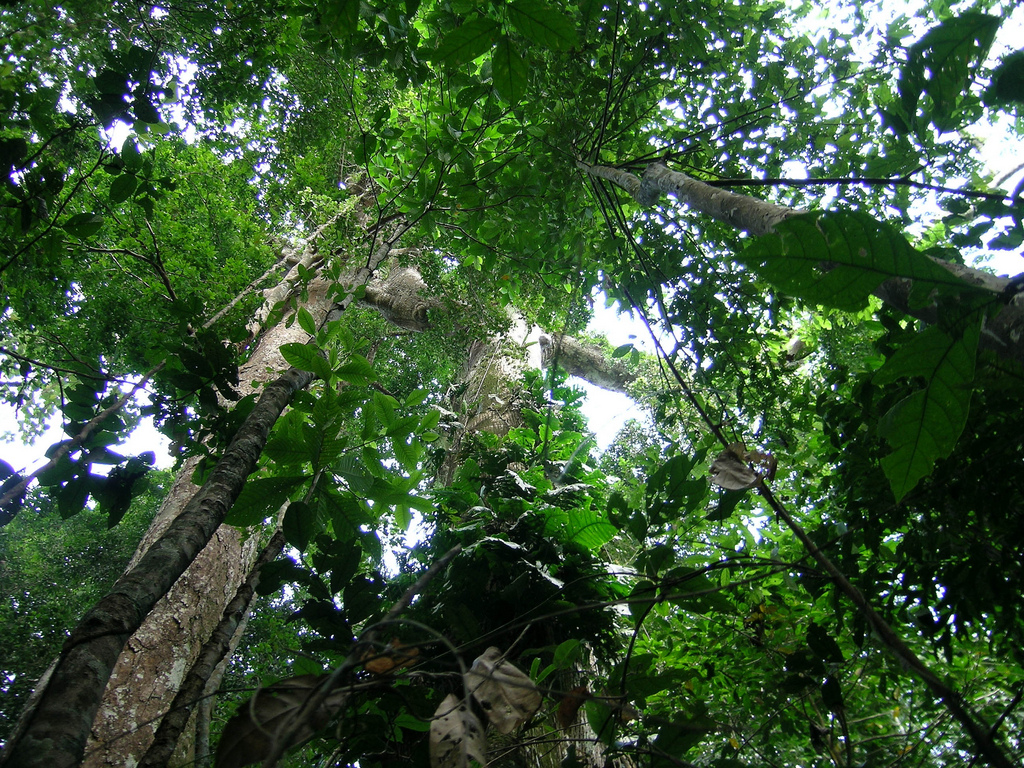
\includegraphics[width=1.0\paperwidth]{images/Background.jpg}}
  \begin{frame}[plain] 

  \begin{TitleBox}
  {\huge \inserttitle}
  \end{TitleBox}

   \begin{TitleBox}
    \insertauthor \\[\baselineskip]
%    \insertshortauthor \\[\baselineskip]
%    \insertshortinstitute
     \insertinstitute   
   \end{TitleBox}

  \end{frame}
}




%-----------------------------------
\end{document}